\section[Lezione 13 - Stabilità dell'interpolazione]{Lezione 13 - Formula dell'errore di interpolazione, interpolazione di Chebyshev, costante di Lebesgue e stabilità dell'interpolazione}

Nella lezione precedente abbiamo visto che nell'interpolazione polinomiale c'è un problema sostanziale di possibile \uline{non convergenza}, che dipende dalla distribuzione dei nodi di campionamento e purtroppo si manifesta proprio con una delle distribuzioni più semplici e usuali nella pratica sperimentale: i \uline{nodi equispaziati} (esempio di Runge).\\
Finora però non abbiamo fornito stime dell'errore di interpolazione, e in particolare della distanza
\[dist \left(f,\inter_n \right) = \max_{x \in [a,b]}\, \abs*{\,f(x) - \inter_n(x)\,}\]
dove $f \in C[a,b]$ e $\inter_n$ è il polinomio interpolatore di grado $\le n$ su $n+1$ nodi distinti in $[a,b]$.\\
A questo proposito, enunciamo e dimostriamo qui sotto un classico risultato di rappresentazione.

\subsection{TEOREMA}
\textbf{(rappresentazione di $f(x) - \inter_n(x)$ per $f \in C^{\,n+1}[a,b]$)}
\begin{center}
    \fbox{\begin{minipage}[t]{15cm}
        Siano $f \in C^{\,n+1}[a,b]$ e $\inter_n \in \mathbb{P}_n$ il polinomio interpolatore su $n+1$ nodi distinti $\{x_i\} \subset [a,b]$, 
        allora 
        \[ E_n(x) = f(x) - \inter_n(x) = \frac{f^{(n+1)}(\xi)}{(n+1)!} \omega_{n+1}(x)\]
        dove
        \[\begin{split}
            \omega_{n+1}(x) & = \prod_{i=0}^n (x-x_i) \\
            & = (x-x_0)(x-x_1)\dotso(x-x_n)
        \end{split}\]
        e $\xi \in int(x, x_0, \dotso, x_n)$ (il più piccolo intervallo aperto che contiene tutti i nodi e $x$ fissato in $[a,b]$).
    \end{minipage}}
\end{center}
Prima di dimostrare il teorema, ricordiamo che possiamo sempre pensare di aver ordinato i nodi in modo che $a \leq x_0 < x_1 < \dotso < x_n \leq b$, ma che non è detto che $x_0 = a$ oppure che $x_n = b$ (come accade invece coi nodi equispaziati).\\
Si noti la somiglianza col resto della formula di Taylor (centrata in $\overline{x}$) nella forma di Lagrange
\[ f(x) - \underbrace{t_n(x)}_{\underset{\text{di Taylor}}{\text{polinomio}}} = \frac{f^{(n+1)}(z)}{(n+1)!} (x - \overline{x})^{n+1}, \ \ z \in int(x, \overline{x}) \]
con la differenza che Taylor ha carattere locale mentre l'interpolazione ha carattere globale e al posto di $(x-\overline{x})^{n+1}$ con $x$ in un intorno di $\overline{x}$, compare $\prod_{i=0}^{n} (x-x_i)$ con $x$ che varia in $[a,b]$.\\
\\
\begin{proof}[\unskip\nopunct]
\uline{Dimostrazione} (facoltativa)\\
Fissiamo $x \notin \left\{ x_0, x_1, \dots, x_n \right\}$: infatti se $x=x_i$ è uno dei nodi $f(x_i) - \inter_n (x_i) = 0$ e $\omega_{n+1}(x_i)=0$ perché i nodi sono proprio gli zeri di $\omega_{n+1}(x)$ che è un polinomio di grado $n+1$.\\
Chiamiamo $E_n(x) = f(x) - \inter_n (x)$ (è in effetti l'errore non in modulo ma col segno nel punto $x$), si noti che $E_n \in C^{n+1}[a,b]$, e definiamo la funzione ausiliaria di variabile $z$
\[ g(z) = E_n(z) - \omega_{n+1}(z) \frac{E_n(x)}{\omega_{n+1}(x)}, \quad z \in [a,b] \]
Ora, $g(x) = 0 = g(x_0) = \dotso = g(x_n)$ (visto  che $E_n(x_i) = 0 = \omega_{n+1}(x_i)$). Quindi la funzione $g$ si annulla in $n+2$ punti in $[a,b]$ che sono gli estremi di $n+1$ intervalli
\begin{center}
    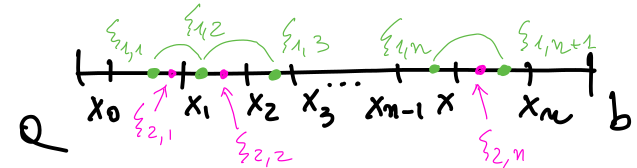
\includegraphics[scale=0.5]{foto/img1_pag6}
\end{center}
(nel disegno abbiamo per esempio $x \in (x_{n-1}, x_n)$).\\
Ricordiamo il \uline{teorema di Rolle} (uno dei risultati cardine del calcolo differenziale in 1 variabile):

\subsubsection{TEOREMA (di Rolle)}
\begin{center}
    \fbox{\begin{minipage}[t]{15cm}%
        Se $\phi \in C[\alpha,\beta]$ è derivabile in $(\alpha,\beta)$ e $\phi(\alpha) = \phi(\beta)$
        \begin{equation*}
            \Rightarrow \exists z \in (\alpha, \beta) : \phi '(z) = 0
        \end{equation*}
    \end{minipage}}
\end{center}
La dimostrazione di basa sul fatto che o $\phi$ è costante in $[\alpha,\beta]$, oppure il max assoluto oppure il min assoluto sono nell'intervallo aperto $(\alpha,\beta)$ e lì la derivata si annulla (la tangente in un punto estremale interno è orizzontale). \\
Allora per il teorema di Rolle applicato a $g$ esistono $n+1$ punti, diciamo $\xi_{1i}, \ 1 \leq i \leq n+1$, ognuno interno ad uno degli intervallini, tali che $g'(\xi_{1i})=0$ (notiamo che $\left\{ \xi_{1,i} \right\} \subset int(x,x_0,\dots,x_n)$). \\
In questo modo sono determinati $n$ intervallini con estremi i punti $\xi_{1,i}$ (si vede il disegno) dove $g'$ si annulla: applicando di nuovo il teorema di Rolle a $g'(x)$ esistono $n$ punti $\xi_{2,i}, \ 1 \leq i \leq n$, ciascuno interno a uno degli $n$ intervallini determinati dai punti $\left\{ \xi_{1,i} \right\}_{1 \leq i \leq n+1}$, tali che $g''(\xi_{2,i}) = 0$ (si noti che $\left\{ \xi_{2,i} \right\} \subset int(\xi_{1,1},\dots, \xi_{1,n+1}) \subset int(x,x_0,\dots,x_n)$). \\
Applicando ripetutamente il teorema di Rolle a $g'',g''',\dotso$, arriviamo infine a dire che $\exists \xi = \xi_{n+1,1} \in int(x,x_0,\dots,x_n)$ tale che $g^{(n+1)}(\xi) = 0$ ma
\[\begin{split}
    g^{(n+1)}(z) & = E_n^{(n+1)}(z) - \omega_{n+1}^{(n+1)}(z) \frac{E_n(x)}{\omega_{n+1}(x)} \\
    & = f^{(n+1)}(z) - (n+1)!\, \frac{E_n(x)}{\omega_{n+1}(x)}
\end{split}\]
perché $\inter_n^{(n+1)}(z) = 0 \,\,\forall\,z$ visto che $\inter_n \in \mathbb{P}_n$ e $\omega_{n+1}^{(n+1)}(z) = (n+1)!$ visto che $\omega_{n+1}(z) = z^{n+1} + \dotso$ (da cui $\omega'_{n+1}(z) = (n+1)z^n + \dotso,\, \omega''_{n+1}(z) = (n+1)nz^{n+1} + \dotso,\,\dotso$).\\
Quindi $\exists \, \xi \in int(x,x_0,\dotso,x_n)$ tale che
\[f^{(n+1)}(\xi) - (n+1)!\frac{E_n(x)}{\omega_{n+1}(x)} = 0\]
che è la rappresentazione cercata.
\end{proof}

\subsection{Stime dell'errore}
Grazie alla rappresentazione esplicita di $E_n(x)$, siamo ora in grado di fare delle stime di
\[\max_{x \in [a,b]} \abs{E_n(x)} = dist\left(f, \inter_n\right)\]
Innanzitutto osserviamo che
\[f \in C^{\,n+1}[a,b] \Longrightarrow f^{(n+1)} \in C[a,b]\]
e quindi per il teorema di Weierstrass sull'esistenza di $max$ e $min$ assoluti di una funzione continua su un intervallo chiuso e limitato
\begin{equation}
    \abs*{f^{(n+1)}(\xi)} \le \max_{x \in [a,b]} \abs*{f^{(n+1)}(x)} = M_{n+1}
\end{equation}
Inoltre comunque $\abs{x-x_i} \le b-a$ quindi
\begin{equation}
    \abs*{\omega_{n+1}(x)} \le (b-a)^{n+1}
\end{equation}
(che è una stima rozza ma valida per qualsiasi distribuzione dei nodi).\\
Quindi in generale possiamo scrivere
\[dist\left(f,\inter_n \right)= \dfrac{f^{n+1}(\xi)}{(n+1)!} \omega_{n+1}(x) 
\overset{(1)}{\leq} M_{n+1} \dfrac{\omega_{n+1}(x)}{(n+1)!} \overset{(2)}{\leq} \overbrace{M_{n+1} \frac{(b-a)^{n+1}}{(n+1)!}}^{stima}\]
Ora, la presenza del fattoriale a denominatore ci potrebbe far sperare che la stima $\to 0,\, n \to \infty$, per $f \in C^{\infty}[a,b]$ (visto che allora la rappresentazione e la stima sono valide $\forall n$): in effetti
\[\frac{(b-a)^{n+1}}{(n+1)!} \to 0, \quad n \to \infty\]
perché è il termine generale della serie di $e^{b-a}$ che converge.\\
Ma sappiamo dall'esempio di Runge che ci sono casi in cui
\[dist\left(f,\inter_n \right) \to \infty, \quad n \to \infty\]
In effetti può succedere che il fattore $M_{n+1}$ nella stima sia non limitato e cresca più rapidamente di 
\[ \frac{(n+1)!}{(b-a)^{n+1}} \]
per $n \to \infty$, cosicché la stima stessa diverge.\\
Infatti è quello che accade (e deve accadere) nell'esempio di Runge (dove l'errore $max$ diverge e quindi la stima diverge).\\
Nel caso dei \uline{nodi equispaziati} si può ricavare una stima più accurata (dimostrazione non richiesta), cioè
\[dist\left(f,\inter_n \right) \le M_{n+1} \frac{h^{n+1}}{4(n+1)}\]
dove $h = \frac{(b-a)}{n}$, ma di nuovo quello che conta è la velocità di crescita di $M_{n+1}$ (che nel caso dell'esempio di Runge cresce più rapidamente addirittura di $(n+1) \cdot h^{-(n+1)}$).\\
La stima ottenuta però ci fa anche capire che ci sono funzioni particolari per cui l'interpolazione sarà sempre convergente, per qualsiasi distribuzione dei nodi (equispaziati, random, sparsi, $\dotso$).\\
Infatti se una funzione $C^{\infty}[a,b]$ ha ad esempio tutte le \uline{derivate equilimitate} (cioè limitate in modulo dalla stessa costante, ovvero $\exists M : M_n \le M \, \forall n$) allora
\[dist\left(f,\inter_n \right) \le M \frac{(b-a)^{n+1}}{(n+1)!} \underset{n \to \infty}{\longrightarrow} 0\]
Esempi sono:
\begin{itemize}
    \item $f(x)=e^x$ per cui $\abs*{f^{(n+1)}(x)} = e^x \le e^b \quad \forall x \in [a,b]$
    \item $f(x)=\sin (x)$ e $f(x)=\cos (x)$ per cui $\abs*{f^{(n+1)}(x)}$ è $\abs*{\sin(x)}$ oppure $\abs*{\cos(x)}$ e quindi $M_{n+1} \le 1$
\end{itemize}
L'esistenza di questi casi $C^{\infty}$ e ``fortunati" non risolve però il problema della convergenza, visto che vorremmo avere un metodo di interpolazione che permetta di approssimare bene funzioni abbastanza generali.

\subsection{Nodi di Chebyshev}
Come abbiamo anticipato, volendo usare un unico polinomio interpolatore $\inter_n$, è necessario cercare distribuzioni speciali dei nodi (visto che i nodi equispaziati, ma anche nodi random o nodi ``scattered" (sparsi) soffrono di situazioni di non convergenza).\\
A questo proposito consideriamo la seguente famiglia di nodi in $[a,b]=[-1,1]$
\begin{center}
    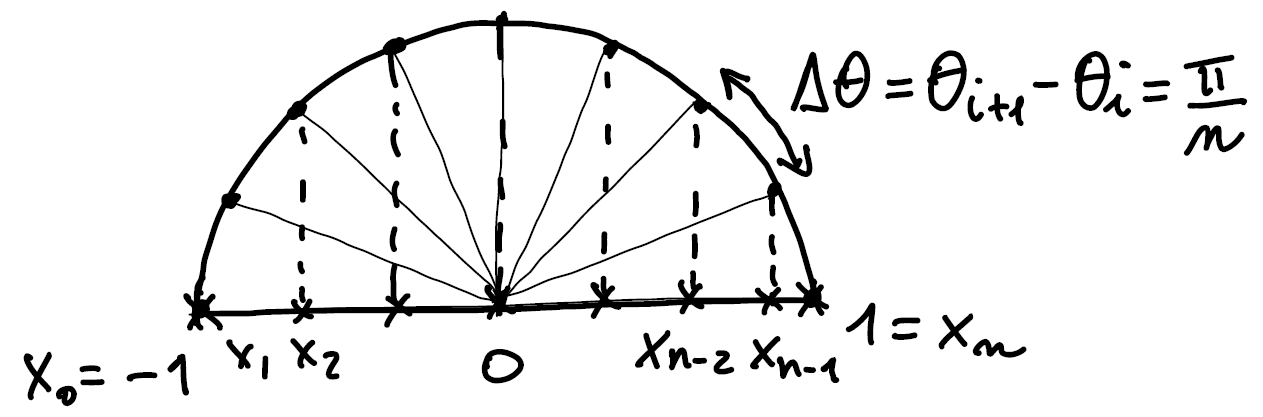
\includegraphics[scale=0.5]{foto/pag-16}
\end{center}
Questi nodi sono ottenuti da punti equispaziati sulla semi-circonferenza di centro (0,0) e raggio 1, cioè corrispondenti agli angoli 
\[\theta_i=i\cdot \frac{\pi}{n}, \quad 0\leq i\leq n,\] 
con 
\[\begin{split}
    \theta_0 & = 0, \\
    \theta_1 & = \frac{\pi}{n}, \\
    \theta_2 & = \frac{2\pi}{n}, \\
    & \dotso \\
    \theta_n & = \frac{n\pi}{n}=\pi,
\end{split}\]
 proiettandoli sull'intervallo $[-1,1]$.\\ 
 Si tratta quindi di coseni 
\[ t_i^{Cheb}=-\cos(\theta_i)=-\cos\left(\frac{i\pi}{n}\right),\quad 0\leq i\leq n \]
(il segno viene cambiato per avere $-1=t_0< t_1<\dotso<t_n=1$) che per costruzione non sono equispaziati ma si addensano  più rapidamente agli estremi dell'intervallo al crescere di $n$ e si chiamano \uline{nodi di Chebyshev} (dal nome del matematico russo che studiò tra i primi il problema dell'interpolazione e approssimazione polinomiale di funzioni continue nel XIX secolo).\\ 
Si può dimostrare (ma la dimostrazione è molto difficile e fa parte di un'intera teoria dell'approssimazione con polinomi) che l'interpolatore su questi nodi, che chiameremo $\inter_n^{Cheb}$, converge uniformemente se $f\in C^k[-1,1]$ per $k>0$, cioè
\[ dist(f,\inter_n^{Cheb})\rightarrow 0 \quad n\rightarrow\infty \]
Per un intervallo generale $[a,b]$ il risultato resta valido se si prendono i nodi ottenuti dalla trasformazione affine
\[ \alpha(t)=\frac{b-a}{2}\cdot t+\frac{b+a}{2},\ \ t\in[-1,1] \]
che manda $[-1,1] \rightarrow [a,b]$, cioè i nodi $x_i^{Cheb}=\alpha(t_i^{Cheb})$ (geometricamente, corrispondono alla stessa costruzione di prima fatta con la semicirconferenza centrata nel punto medio dell'intervallo, $\frac{b+a}{2}$, e di raggio la semilunghezza dell'intervallo, $\frac{b-a}{2}$).\\
In effetti si riesce anche a dare l'ordine di infinitesimo in $n$ per $k$ fissato

\subsection{TEOREMA (convergenza uniforme dell'interpolazione di Chebyshev)}
\begin{center}
    \fbox{\begin{minipage}[t]{15cm}%
        Sia $f \in C^k[a,b], \, k > 0$, 
        allora 
        \[ \exists \, c_k>0 : dist \left(f, \inter_n^{Cheb} \right) \le c_k \frac{\log (n)}{n^k}\]
    \end{minipage}}
\end{center}
Si osservi che 
\[ \frac{\log (n)}{n^k} \to 0, \quad n \to \infty, \quad \forall \, k > 0 \]
più velocemente più grande è $k$; si può far vedere che $c_k$ è proporzionale a 
\[\max_{x \in [a,b]} \abs*{f^{(k)}(x)} \quad \text{(Teorema di Jackson)}\]
È chiaro che se $f$ è almeno $C^1$ (esistono esempi di funzioni solo continue per cui l'interpolazione di Chebyshev non converge) con i nodi di \uline{Chebyshev} abbiamo \uline{risolto} il problema della \uline{convergenza uniforme} dell'interpolazione polinomiale.\\
È il caso di ricordare che esistono altre famiglie di nodi tipo Chebyshev, per cui vale un teorema tipo quello enunciato sopra.\\
Si tratta di nodi non equispaziati che si addensano più rapidamente agli estremi con una legge tipo coseno (non basta prendere nodi non equispaziati e neppure nodi che si addensano agli estremi al crescere di $n$, la chiave è il modo in cui si addensano).\\
Un'altra famiglia, ad esempio, è
\[x_i^{Cheb2} = \alpha(t_i^{Cheb2})\] con
\[t_i^{Cheb2} = - \cos{\left(\frac{\pi}{2}\cdot \frac{2i+1}{n+1}\right)}, \quad 0 \le i \le n\]
(si noti che mentre la prima famiglia comprende gli estremi dell'intervallo, $x_0^{Cheb}=a$ e $x_n^{Cheb}=b$, qui $x_0^{Cheb2}>a$ e $x_n^{Cheb2}<b$, cioè i nodi pur addensandosi agli estremi stanno in $(a,b)$).\\
Dopo aver discusso il problema della convergenza, resta da affrontare un altro problema che sorge in modo naturale, quello della \uline{stabilità} dell'interpolazione polinomiale.\\
Infatti, i valori della funzione campionata in pratica non sono mai noti in modo esatto, ma sono sempre affetti da errori (di arrotondamento, di misura sperimentale, $\dotso$).\\
Supponiamo quindi di avere a disposizione non gli $\{y_i\}$ ma dei valori approssimati $\{\Tilde{y}_i\}$ e di avere una stima dell'errore, del tipo
\[\max_{0 \le i \le n} \abs*{\,\Tilde{y}_i - y_i\,} \le \varepsilon\]
Quindi il polinomio interpolatore sarà $\Tilde{\inter}_n(x)$ invece di $\inter_n(x)$.

\subsection{Convergenza e stabilità del polinomio interpolatore}
La domanda è: come risponde l'interpolatore agli errori sui dati?\\
Quello che dobbiamo fare è una stima di $dist \left(\inter_n, \Tilde{\inter}_n \right)$ per capire come dipenda da $\varepsilon$ (e da $n$).\\
Ci viene in aiuto la forma di Lagrange, per cui l'interpolatore ``esatto" è
\[\inter_n(x) = \sum_{i=0}^n y_i \, l_i(x), \quad y_i = f(x_i)\]
mentre l'interpolatore ``perturbato" (quello costruito coi valori affetti da errore, gli unici che abbiamo veramente a disposizione) è
\[\Tilde{\inter}_n(x) = \sum_{i=0}^n \Tilde{y}_i \, l_i(x)\]
Allora
\[\begin{split}
    \abs*{\,\inter_n(x) - \Tilde{\inter}_n(x)\,} & = \abs*{\,\sum_{i=0}^n y_i \, l_i(x) - \sum_{i=0}^n \Tilde{y}_i \, l_i(x)\,} \\
    & = \abs*{\,\sum_{i=0}^n (y_i - \Tilde{y}_i)\, l_i(x) \,} \\
    & \le \sum_{i=0}^n \overbrace{\abs*{\,y_i - \tilde{y}_i\,}}^{\le\, \varepsilon}\, \abs{\,l_i(x)\,} \\
    & \le \varepsilon \sum_{i=0}^n \abs{\,l_i(x)\,}, \quad \forall\, x \in [a,b]
\end{split}\]
La funzione 
\[\lambda_n(x) = \sum_{i=0}^n \abs*{\,l_i(x)\,}\]
si chiama funzione di Lebesgue: non è un polinomio, ma è la somma di moduli di polinomi (i polinomi elementari di Lagrange) ed è solo continua in $[a,b]$, perché gli zeri di $l_i(x)$ in $(a,b)$, cioè i nodi $\{x_j \in (a,b) : j \ne i\}$, sono punti ``angolosi" (cioè punti di non derivabilità di $\abs{\,l_i(x)\,}$, per cui $\abs{l_i}\in C[a,b]$ ma $\abs{l_i} \notin C^1[a,b]$
\begin{center}
    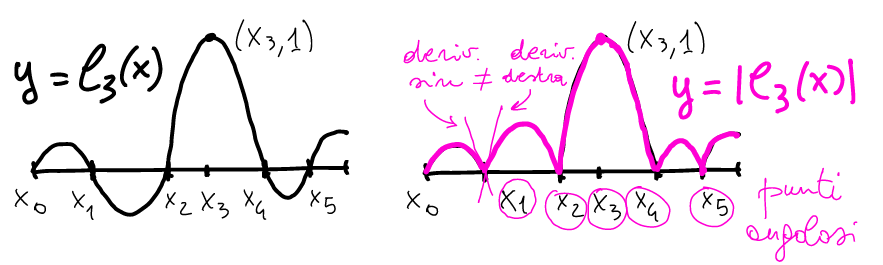
\includegraphics[scale=0.8]{foto/lez13_img2}
\end{center}
Prendendo il max in $[a,b]$ da ambo i lati della disuguaglianza 
\[ \abs*{\inter_n(x)-\tilde{\inter}_n(x)}\leq \varepsilon  \sum_{i=0}^n \abs{l_i(x)}=\varepsilon\lambda_n(x) \]
Si ottiene
\[ dist\left(\inter_n,\tilde{\inter}_n\right)\leq \Lambda_n \]
dove 
\[\Lambda_n= \max_{x\in[a,b]}\lambda_n(x)\]
viene detta \uline{COSTANTE DI LEBESGUE} dei nodi di interpolazione.\\
Si noti infatti che tale quantità (costante in $x$) dipende \uline{solo} dai nodi $\{ x_i \}$ e agisce come un \uline{coefficiente}\\ \uline{di amplificazione} del massimo errore $\varepsilon$ sui dati.\\
Si può dimostrare (ma è difficile) che esistono delle costanti $\alpha_1, \alpha_2, \alpha_3 > 0$ tali che
\begin{enumerate}
    \item $\Lambda_n \geq \alpha_1 log(n)$ per \uline{qualsiasi} distribuzione di nodi
    \item $\Lambda^{eq}_n \sim \alpha_2 \frac{2^n}{nlog(n)}, \ n \to \infty, \ \alpha_2 = \frac{2}{e} \simeq 0.74$
    \item $\Lambda^{Cheb}_n \leq \alpha_3 log(n), \ \alpha_3 \simeq \frac{2}{\pi} \simeq 0.64$
\end{enumerate}
cioè, la costante di Lebesgue cresce almeno come $\log(n)$, ma nel caso dei nodi \uline{equispaziati} ha crescita sostanzialmente \uline{esponenziale}, mentre nel caso delle varie distribuzioni dei nodi di tipo \uline{Chebyshev} ha crescita \uline{logaritmica} e quindi quasi ottimale.\\
La stima ottenuta mostra che l'interpolazione su \uline{nodi equispaziati}, oltre ad essere in generale non convergente, è anche \uline{instabile}, mentre l'interpolazione di \uline{Chebyshev} oltre ad essere convergente (per $f \in C^k, k>0$) è anche sostanzialmente \uline{stabile}, perché $\log(n)$ cresce molto lentamente.\\
Ad esempio per $n=30$ si ha:
\begin{itemize}
\item $\Lambda^{eq}_{30} \simeq 8 \cdot 10^6$
\item $\Lambda^{Cheb}_{30} \lesssim 2.2$
\end{itemize}
e per $n=50$:
\begin{itemize}
\item $\Lambda^{eq}_{50} \simeq 4 \cdot 10^{12}$
\item $\Lambda^{Cheb}_{50} \lesssim 2.49$
\end{itemize}
Questo significa che anche per le classi di funzioni su cui convergerebbe (ad esempio funzioni con derivate ``equilimitate", come visto prima), in pratica l'interpolazione polinomiale su nodi equispaziati è inutilizzabile appena $n$ cresce.\\
Invece l'interpolazione di Chebyshev è un'ottima scelta, visto che partendo dalla disuguaglianza
\[ \abs*{f(x) - \tilde{\inter}_n (x)} \leq \abs*{f(x) - \inter_n (x)} + \abs*{\inter_n (x) - \tilde{\inter (x)}} \]
e prendendo il max in $[a,b]$ da ambo i lati, otteniamo
\[ dist\left(f, \tilde{\inter}_n\right) \leq \underbrace{dist \left(f, \inter_n \right)}_{\text{convergenza}} + \underbrace{dist \left( \inter_n, \tilde{\inter}_n\right)}_{\text{stabilità}} \underbrace{\lesssim}_{\text{per i nodi di Cheb}} c_k \frac{\log(n)}{n^k} + 0.64\cdot \log(n) \cdot \varepsilon \]
se $f \in C^k [a,b], k>0$ e $\max\abs{y_i - \tilde{y_i}} \leq \varepsilon$\\
C'è però uno svantaggio evidente nell'interpolazione di Chebyshev: è necessario interpolare su \uline{quei} particolari nodi per garantire convergenza e stabilità, mentre potrebbe essere più semplice o più naturale campionare su altri nodi (equispaziati, sparsi, $\dotso$).\\
In questi casi cosa si può fare? Vedremo nella prossima lezione che il problema della convergenza (e della stabilità) è risolubile infittendo il campionamento con distribuzioni arbitrarie dei nodi, tramite le tecniche di interpolazione \uline{polinomiale a tratti}.
\newpage
